\documentclass[a4paper,12pt,twoside]{article}	% debut d'un fichier latex standard

\usepackage{graphicx}	% pour l'inclusion de figures en eps,pdf,jpg
\usepackage{amsmath}	% quelques symboles mathematiques en plus
\usepackage{amssymb}
\usepackage{mathrsfs}
%\usepackage{psfrag}

\usepackage{listings}

\usepackage{mathenv}

\usepackage[british,UKenglish,USenglish,english,american]{babel}	
% \usepackage[francais]{babel}	% le tout en langue francaise
% \usepackage[latin1]{inputenc}	% on peut ecrire directement les caracteres avec l'accent(L/W)
\usepackage[colorlinks,bookmarks=false,linkcolor=blue,urlcolor=blue]{hyperref}	% pour l'inclusion de links dans le document 

\paperheight=297mm
\paperwidth=210mm

\setlength{\textheight}{235mm}
\setlength{\topmargin}{-1.2cm} % pour centrer la page verticalement -1.2
%\setlength{\footskip}{5mm}
\setlength{\textwidth}{15cm}
\setlength{\oddsidemargin}{0.2cm}
\setlength{\evensidemargin}{0.56cm}

\pagestyle{plain}

% quelques abreviations utiles
\def \be {\begin{equation}}
\def \ee {\end{equation}}
\def \bs {\begin{equation} \left\{  \begin{aligned}}
\def \es {\end{aligned} \right. \end{equation}}
\def \dd  {{\rm d}}
\def \un {\,\,\mathrm}


\newcommand{\mail}[1]{{\href{mailto:#1}{#1}}}
\newcommand{\ftplink}[1]{{\href{ftp://#1}{#1}}}


% ======= Le document commence ici ======
\begin{document}

% Le titre, l'auteur et la date
\title{Optical tweezer}
\date{\today}
\author{
	% Laurent \bsc{Rohrbasser}\\{\small \mail{laurent.rohrbasser@epfl.ch}} \and 
	% Tim \bsc{Tuuva}\\{\small \mail{tim.tuuva@epfl.ch}}
	Laurent Rohrbasser\\{\small \mail{laurent.rohrbasser@epfl.ch}} \and 
	Tim Tuuva\\{\small \mail{tim.tuuva@epfl.ch}}
	}
\maketitle

\tableofcontents % Table des matieres

% Quelques options pour les espacements entre lignes, l'identation 
% des nouveaux paragraphes, et l'espacement entre paragraphes
\baselineskip=16pt
\parindent=15pt
\parskip=5pt

% \section{Abstract}
\begin{abstract}

This document will show the results got on an implementation of the lowcost optical tweezer decribed in the paper called "Inexpensive optical tweezers for undergraduate laboratories". The goal is to see how well that experiments works on simple shapes such as tiny dielectric spheres in water by looking at their position through time while trapped and not trapped.

\end{abstract}

\section{Introduction}
In 1970, Arthur Ashkin did build the first tool that could control a tiny object's position without touching it using a laser beam in Bell labs. It was the first implementation of what we call now an optical tweezer, a tool that is commonly used in a lot of domains where it is needed to manipulate precisely some small objects (eg. moving cells in biology). An optical tweezer is a focused beam of light that can hold microscopic particles in three dimensions. This tool can apply an attractive or a repulsive force on any dieletric objects. 


\section{Theory}
There are different phenomena that applies, depending on the size of the dieletric objects, to explain the trapping force.
If the objects is much smaller than the laser wavelenght we use the electric dipole model.
If the objects is much bigger than the laser wavelenght we explain the trapping by the refracting force and the momentum conservation.
This experiment uses a red HeNe laser light with a $658 nm$ wavelenght and the smallest objects size is $0.5\mu m$,
therefore we will focus on the optic approach.
\begin{figure}[h!]
	\begin{center}
	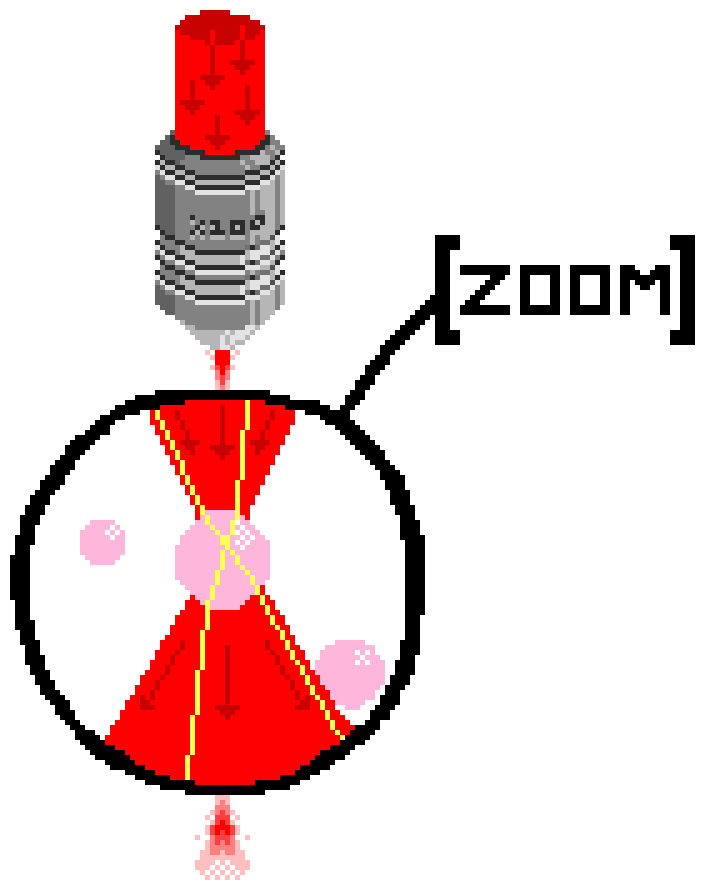
\includegraphics[width=0.5\linewidth,angle=0]{./figures/lazor_zoom}
	\caption{The laser is focused on one point, a particle that gets some rays through it refracts them, and momentum conservation conduct them to be attracted to a point near the focus point.} \label{fig:theory}
	\end{center}
\end{figure}


The individual rays of light (from the laser) are refracted at the interface of the dieletric, when they enter and leave it.
Since light is associated with a momentum, one can notice that its momentum change when its direction changes.
By applying the third law of Newton and the conservation of momentum, the momentum of light is transfered to the particle when the ray is refracted.
As the laser is aligned on the microscope axis, the trapping force is greater on this axis because
 the refraction is greater as the particle is far from the axis and practically inexistant if the particle is perfectly aligned on the axis.
The beam is also focused by the objective lens, thus, the same argument applies on the z axis.

The paper "Inexpensive optical tweezers for undergraduate laboratories" gives an example of the kind of profile we get for the force applied on the particle depending on z : fig \ref{fig:force_prof}

\begin{figure}[h!]
	\begin{center}
	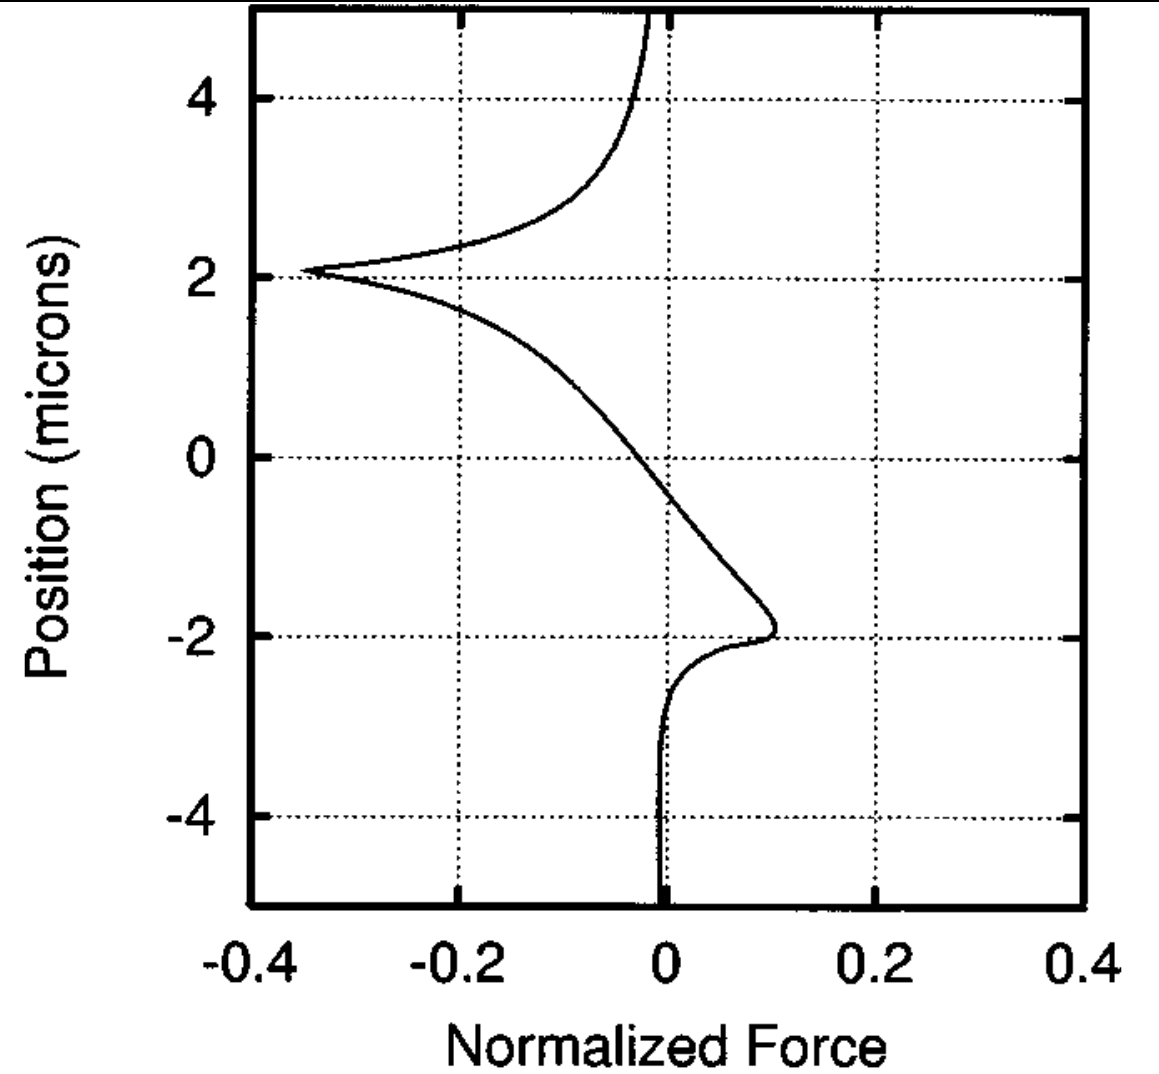
\includegraphics[width=0.5\linewidth,angle=0]{./figures/force_profile}
	\caption{The particle should stabilize lower than the point where the beam is focused} \label{fig:force_prof}
	\end{center}
\end{figure}



% \clearpage

\section{Dispositif}
There are two main parts to build an optical tweezer:
\begin{itemize}
	\item Microscope
	\item Laser system
\end{itemize}

\subsection{Microscope}
It is made of an objective and an ocular lens. A lamp enlights the sample placed in the focal plane of the objective lens which enlarge the observed object (x100 in our case). A shortpass filter that reflects only one kind of electromagnetic wave (one wavelength) is used as a filter : it is placed between the objective and the lens to filter out the laser beam reflected from the sample plate by reflecting it back on the plate. Finally, the ocular lens focus the objective image into the CCD camera which shows us the image on a monitor screen. Experimentally, it has been constated that the last lens had no really other effects than making the final image bigger (and darker) or smaller (and brighter).

\subsection{Laser system}
The laser is sent into the microscope objective using some mirrors and a dichoirc mirror. It reflects the laser beam on one direction and let it pass on the other direction.
Initially, the laser is colimated, but since it is too small one should enlarged it, using 2 lens placed in each other focal plane, thus to create a telescope. Therefore, the laser is enlarged and slightly diverging when arriving into the objective. This particular configuration helps to the trapping force effect.

\begin{figure}[h]
	\begin{center}
		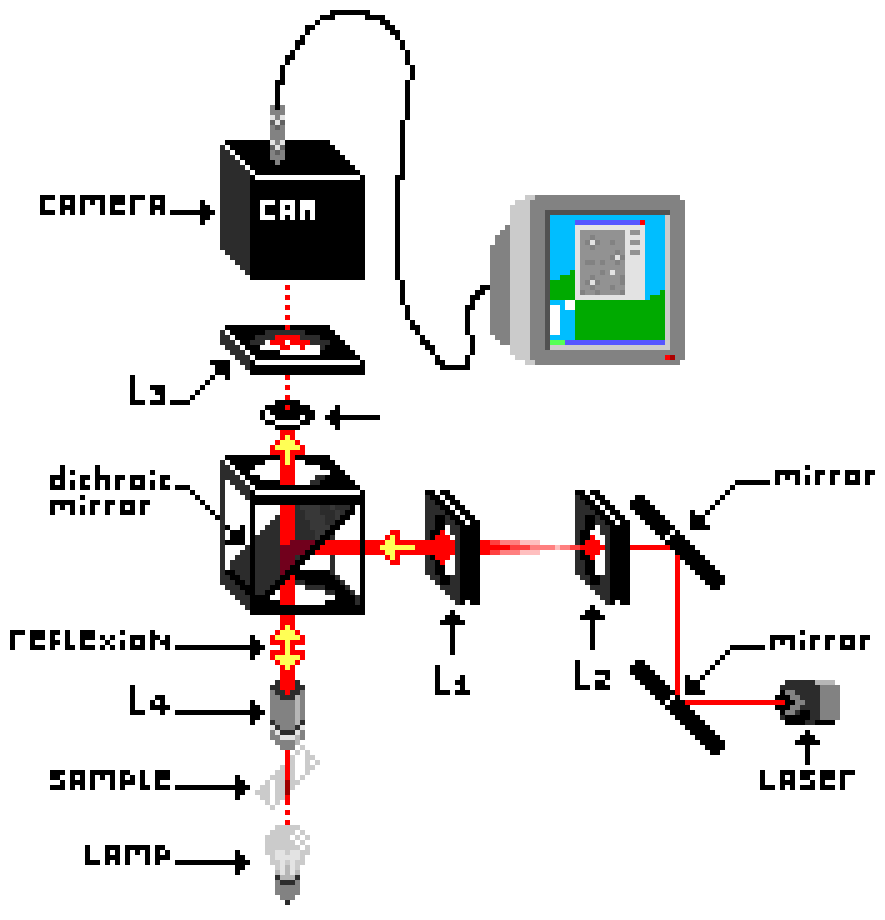
\includegraphics[width=0.8\linewidth,angle=0]{./figures/montage_1}
		\caption{Optical tweezer setup schema.} \label{fig:dispositif}
	\end{center}
\end{figure}

\section{Results}
\subsection{Calibration}
The first task is to calibrate the microscope using a resolution test target (R3L3S1P - Positive 1951 USAF), the results are reasumed in the table~\ref{tab:calibration}

\begin{table}[h!]
\centering
	\begin{tabular}{|c|c|c|c|}
		\hline
		schema & lines pair by milliter[$LP/mm$]& pixel by lines[$Pixel/L$] & [$mm/Pixel$]\\
		\hline
		7.1	& 128.0	& 52 & 7.51e-05\\
		7.2	& 144.0	& 46 & 7.54e-05\\
		7.3	& 161.0	& 41 & 7.57e-05\\
		7.5	& 203.0	& 33 & 7.46e-05\\
		7.6	& 228.0	& 30 & 7.30e-05\\
		\hline
	\end{tabular}
	\caption{Calibration values table}
	\label{tab:calibration}
\end{table}

\subsection{Microscope}

The microscope part did work well. After many observations on serval samples with different concentrations, it was possible to get a $4000 $x zoom with a clear image when the focus was correct. All particles were distinguishable and it was observed that if a partcle moved on z, the focus was easly lost but that did happen slowly, so it was not a big problem to collect data. It had been a delicate task to find the best lighting so that the algorithm of the given software (MOSAIC in imageJ) can detect some particles (the particle had to appear darker or brighter than everything else, the ring shape was not the optimal input).

\subsection{Sample}

The sample is set as follow : a glass plate is put on an other glass plate separated with a small distance fixed by the width of a double faced tape that join those two elements. In the little space created inbetween, a mixture of distilled water with the element we want to trap is put. The volume is set so that particles are free to move but not too much on z, so that it is more controllable in the experiment. cf fig \ref{fig:sample} for an illustration.

\begin{figure}[h]
	\begin{center}
	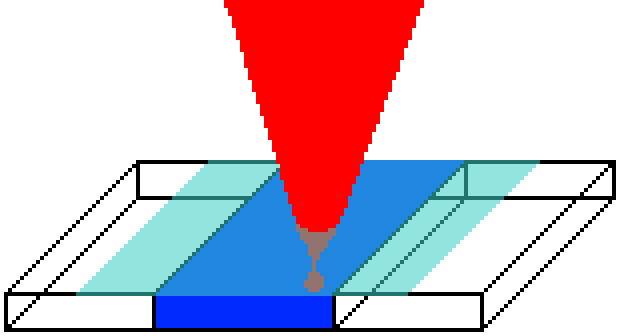
\includegraphics[width=0.7\linewidth,angle=0]{./figures/sample}
	\caption{sample illustration. The dark blue part correspont to the liquid containing elements we want to trap, the ligh blue part is a glass plate, the white elements are the tape, the red thing is the laser that will go throw the sample} \label{fig:sample}
	\end{center}
\end{figure}

\subsection{Trapping}

The trapping part was an other story. All adjustments that were made are based on the observation of the largest particle avaiable for the simple reason that they were the easiest to manipulate.

The installation worked well in a particular case that did not look like the description in the theory.

When the lens were choosed so that they fit the specifications (try to get a bigger beam with a colimated light beam), the force applied on the particles was weak, almost negligeable. It was hard to catch and move a particle in space.

However, when a complety wrong lens was used (L2 had a way too large focal length, something like 1 meter, and L1 had a 5 cm focal length, and the distance between those lens was set to 12 $\pm$ 3 cm), there was an other effect and the laser did catch successfully on x and y. There was a very strong force and it was possile to catch a lot of particles in same time. It was possible to see some particles "fall" from a high z to the focal point (a blurry effect made that easy to intuite).

With a small sheet of paper, it was possible to see how the laser looked like in the line between L4 and the dichroic mirror in the second case : it was almost parallel and slightly growing when approaching the L4 lens, so it was a little bit closer to what was wanted compared to the approximation with the L2 lens that had an infinite focal length for the input, instead of it actual (high) 16 cm.

It was seen that the force was much stronger than in the normal case, but there was a problem : the trapping was working only on x and y, not on z, more details about that is given in the next section. The wrong lens was initially choosen by mistake because all lenses were not put in their correct box. Since it had been constated that there were some better results with those wrong lenses, it had been tried some other configurations of pairs of lenses, in some cases with some random lenses and in some cases with a pair that did fit the specification. It had been seen that the best result was always got by using a lens L2 with a very high focal length, but that the force with the "correct" pair of lens had somme poor attraction (hard to test on x,y and even harder on z). 


\begin{figure}
	\begin{center}
	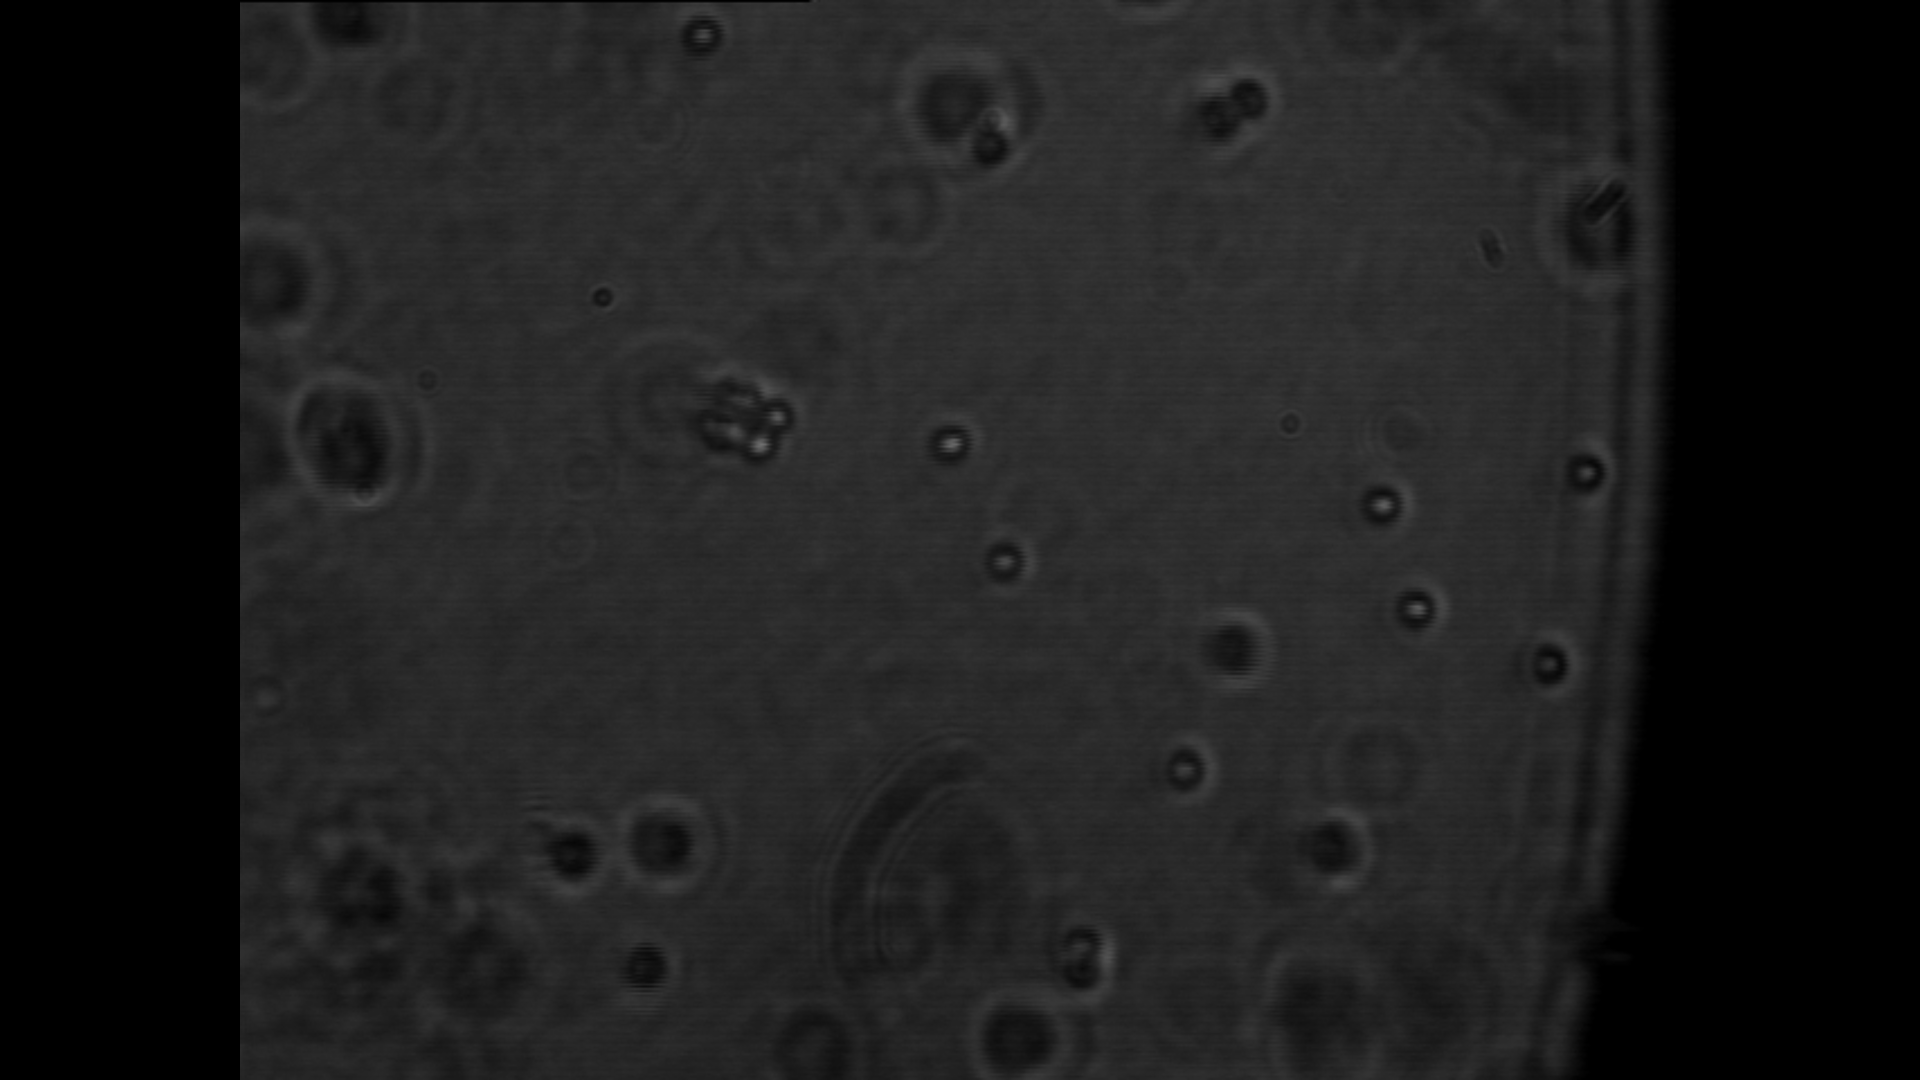
\includegraphics[width=0.7\linewidth,angle=0]{./figures/gros_trap}
	\caption{large particles beeing trapped} \label{fig:gros_trap}
	\end{center}
\end{figure}
\begin{figure}
	\begin{center}
	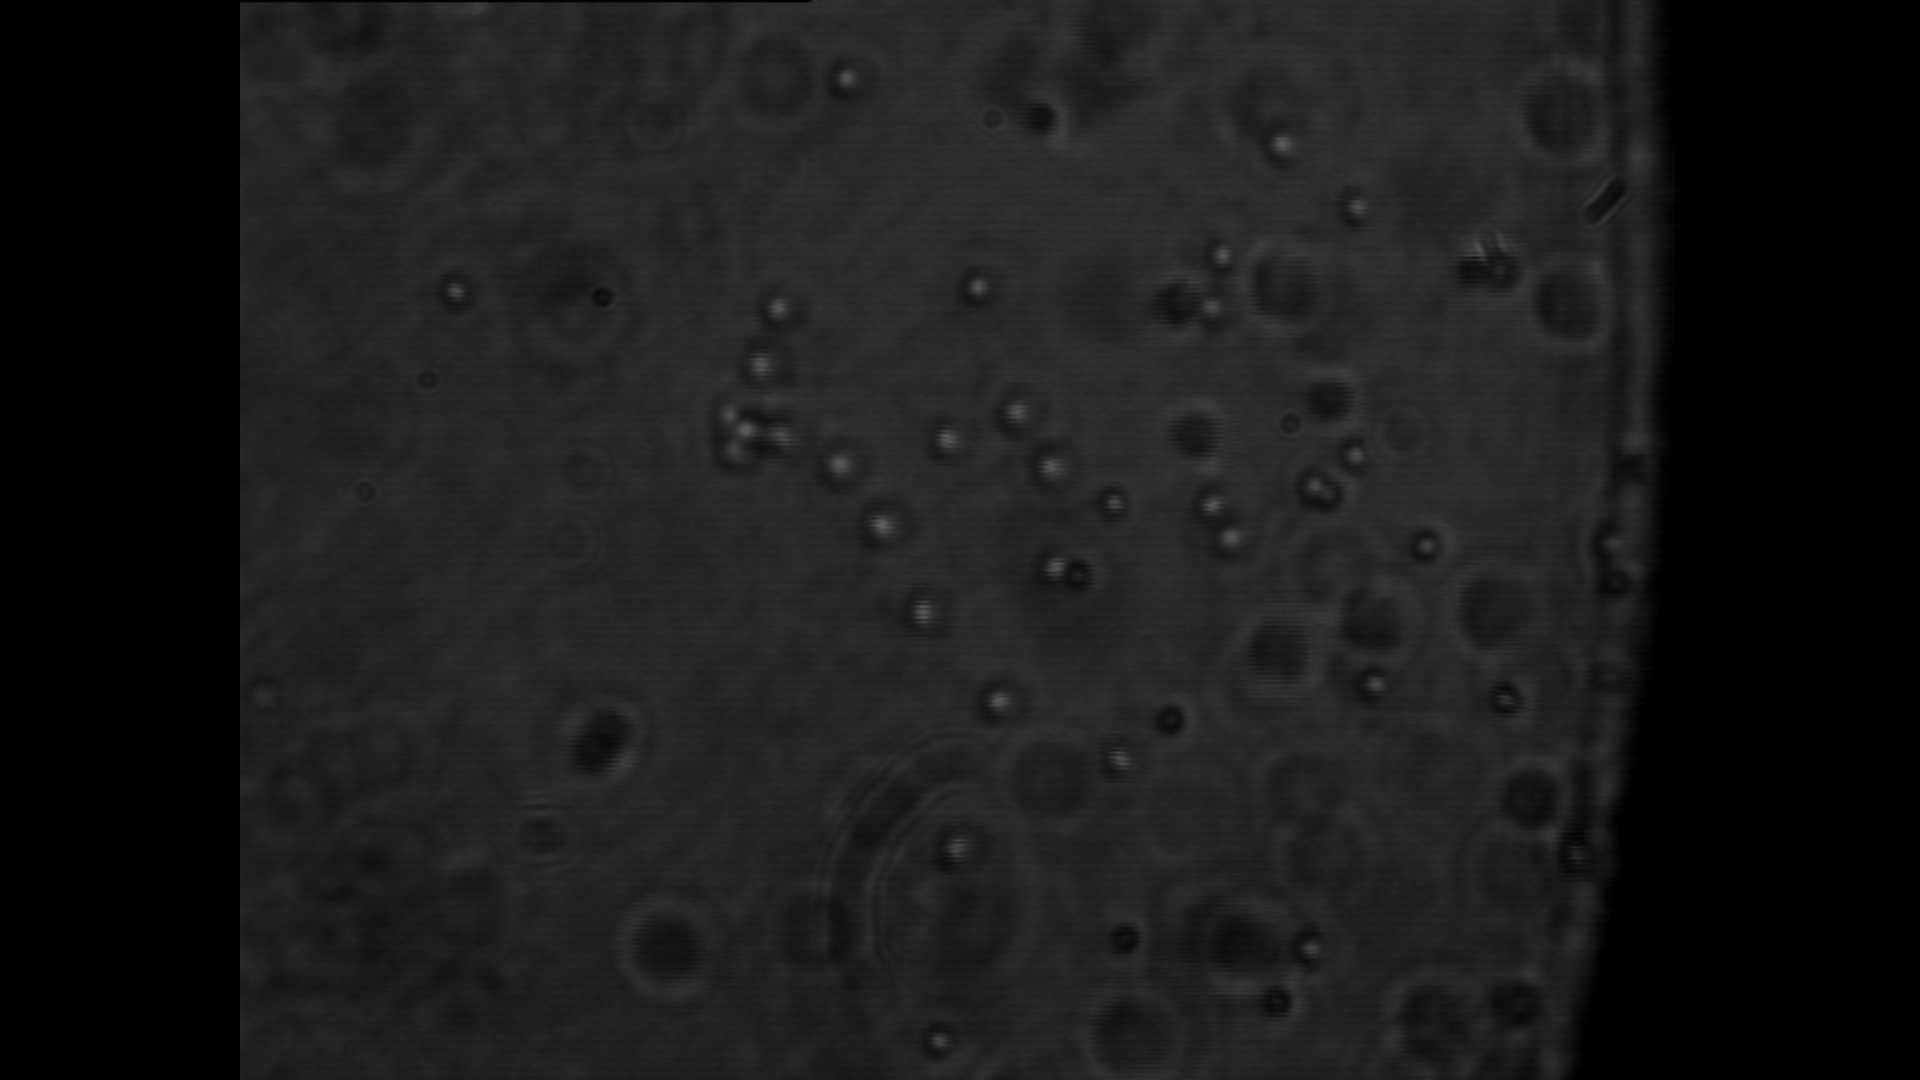
\includegraphics[width=0.7\linewidth,angle=0]{./figures/moyen_trap}
	\caption{medium particles beeing trapped} \label{fig:gros_trap}
	\end{center}
\end{figure}
\begin{figure}
	\begin{center}
	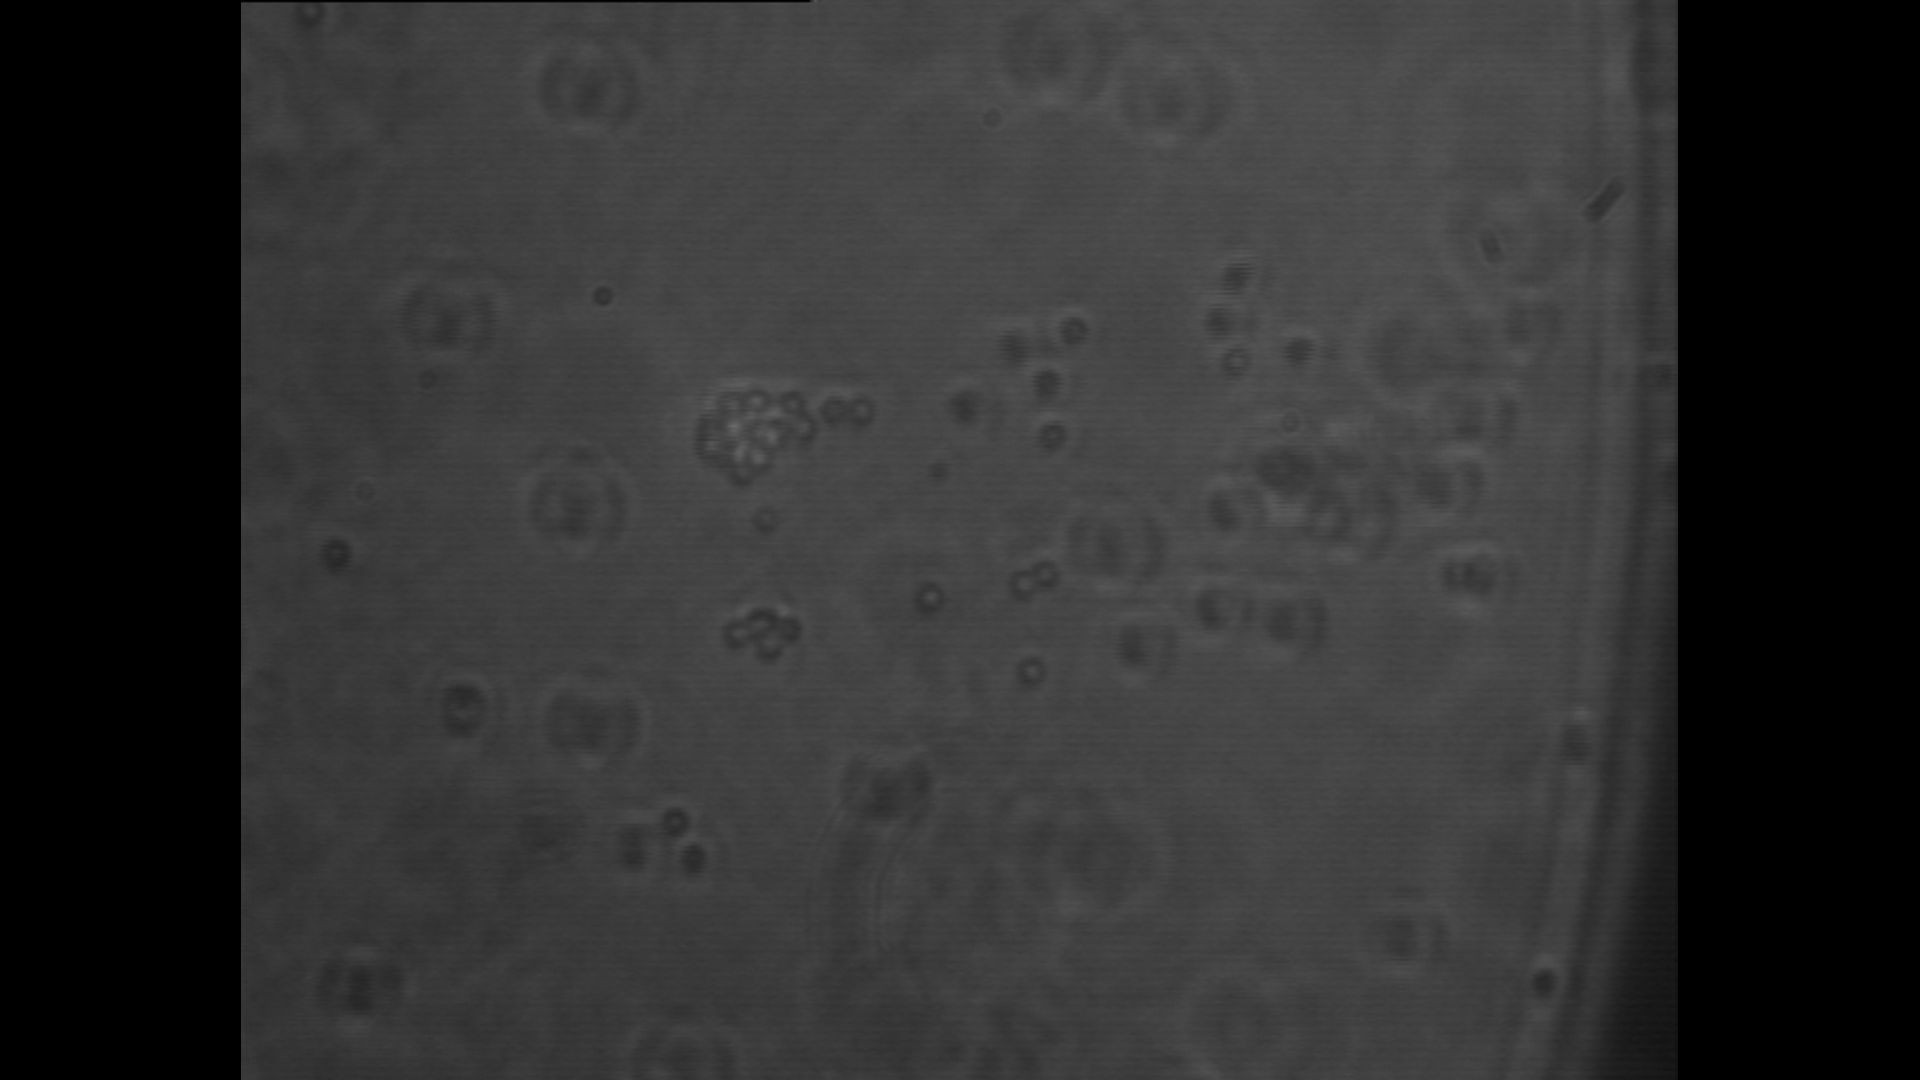
\includegraphics[width=0.7\linewidth,angle=0]{./figures/petit_trap}
	\caption{small particles beeing trapped} \label{fig:gros_trap}
	\end{center}
\end{figure}


\subsection{Tracking}

As shown on the following illustration, no usable data was got from our videos. However, the results show that the trapped particles (even if the tracking has gone wrong) were moving much less that the not trapped ones. It has also been written a C code that treat the data outputted by MOSAIC that can be easily changed to do some calibrations (see attachement).


% ILLUSTRATION DETECTION PARTICULE RING -> GROS CACA

% ILLUSTRATION DETECTION PARTICULE POINT -> TRAJECTOIRE


\begin{table}
	\begin{tabular}{ r|c|c|c| }
		\multicolumn{1}{r}{} &  \multicolumn{1}{c}{Small [$\O 0.5\mu m$]} & 			\multicolumn{1}{c}{Medium [$\O 1.25\mu m$]} & 			\multicolumn{1}{c}{Big [$\O 2.25\mu m$]}\\
		% \cline{2-4}						& 1 & 2 & 3 \\
		%   								& 1 & 2 & 3 \\

		\cline{2-4} Mean $[m^2/s] \Rightarrow$ & ?? & ?? & ??\\
		\cline{2-4} Theory $[m^2/s] \Rightarrow$ & 4.29e-13 & 1.71e-13 & 9.53e-14\\
		\cline{2-4}
	\end{tabular}
	\caption{Table of the Experimental and Theorical values for the diffusion coefficient.}
	\label{tab:diffusion}
\end{table}


\section{Analysis and Discussion}

Here are some more details and our interpretation on the observations done on the effect of the beam on z.

By moving the focus, it was possible to see that particles were trapped when the focus was close the bottom plate : it looked that all particles were trapped in a cone under the focal point. When the focus was near the plate, it was possible to see a clear reflexion of the laser in the plate when the filter was removed, and it was on that moment that the force was at the highest point. When the focal point was moved a bit higher than the plane level, the force got weaker, but it was still possible to trap some particles. All trapped particles looked blury, that meant that they were far from the focal point, and since it was not possible to trap particles on the upper surface of the sample, we deduced that those particles must have been on the bottom of the plate.

It might be a good idea to implement a thing that allows to mesure the distance of a particle using the appearant size of the particle when the focus is not on it.

When the focal point was set quite far away from the plate, and when the experiment was left for a few minutes, it had been seen that there was a big accumulation of particles in a large circle, all of them looking blurry. That unintentionnal experiment made believable that all those particles were attracted on a cone under the focal point like this : they all looked free inside a circle centered on a line going throw the center of the laser beam and pushed down on z. There were no particles closer to the focal point in that experiment.


\begin{figure}
\centering
\begin{minipage}{.5\textwidth}
	\centering
	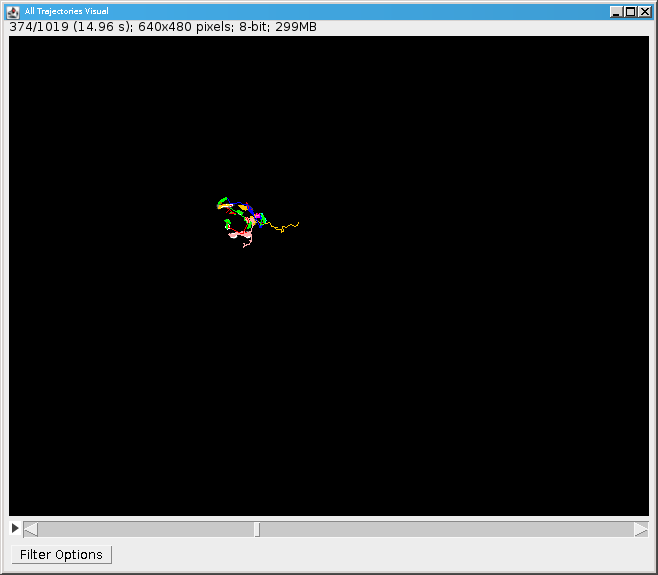
\includegraphics[width=.95\linewidth]{./figures/trapped_traj}
	\caption{trapped particle trajectory, they are spinning on a polygon (they are hold in the same position)}
	\label{fig:test1}
\end{minipage}%
\begin{minipage}{.5\textwidth}
	\centering
	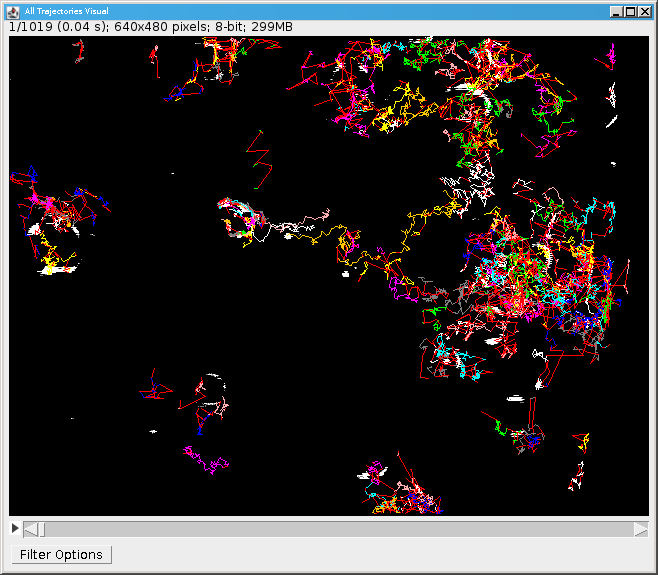
\includegraphics[width=.95\linewidth]{./figures/trapped_traj_2}
	\caption{trajectory of all particles, free particles move much further than the trapped ones.}
	\label{fig:test2}
\end{minipage}
\end{figure}


\begin{figure}
\centering
\begin{minipage}{.5\textwidth}
	\centering
	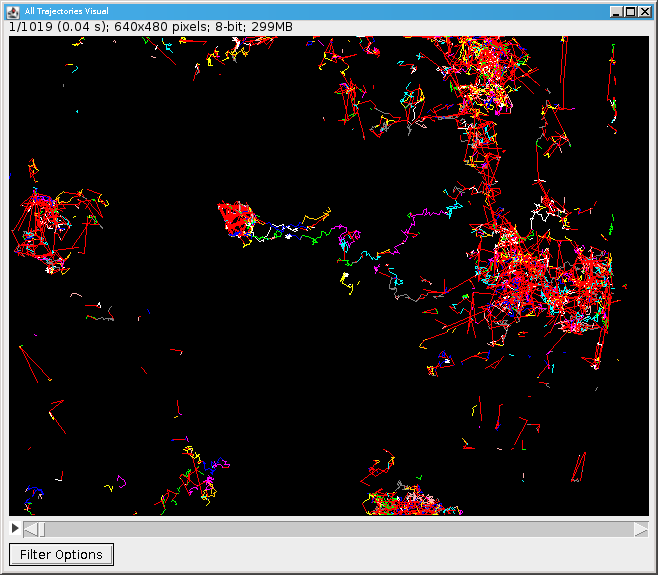
\includegraphics[width=.95\linewidth]{./figures/traj_gros_trap}
	\caption{big particles trapped}
	\label{fig:test1}
\end{minipage}%
\begin{minipage}{.5\textwidth}
	\centering
	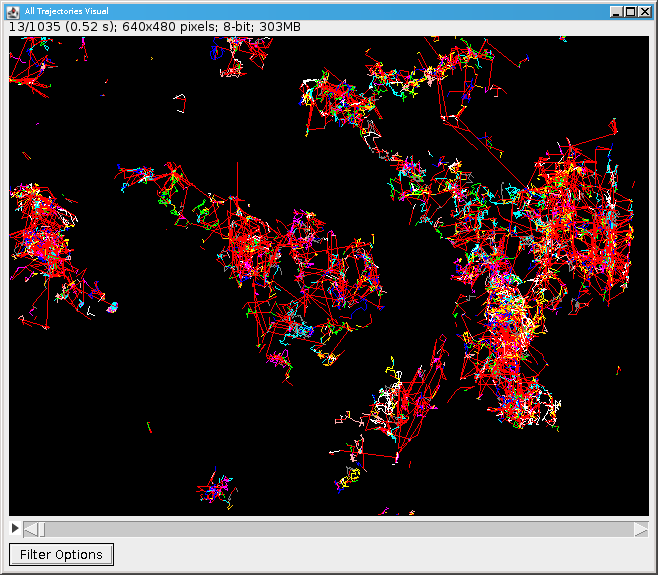
\includegraphics[width=.95\linewidth]{./figures/traj_gros_free}
	\caption{big particles free}
	\label{fig:test2}
\end{minipage}
\end{figure}


\begin{figure}
\centering
% \begin{minipage}{.5\textwidth}
	% \centering
	% \includegraphics[width=.95\linewidth]{./figures/traj_moyen_trap}
	% \caption{middle size particles trapped}
	% \label{fig:test1}
% \end{minipage}%
\begin{minipage}{.5\textwidth}
	\centering
	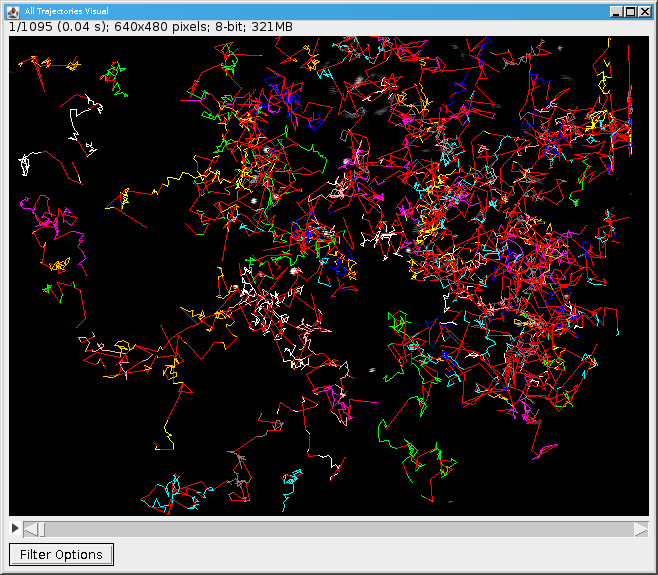
\includegraphics[width=.95\linewidth]{./figures/traj_moyen_free}
	\caption{middle size particles free}
	\label{fig:test2}
\end{minipage}
\end{figure}


\begin{figure}
\centering
\begin{minipage}{.5\textwidth}
	\centering
	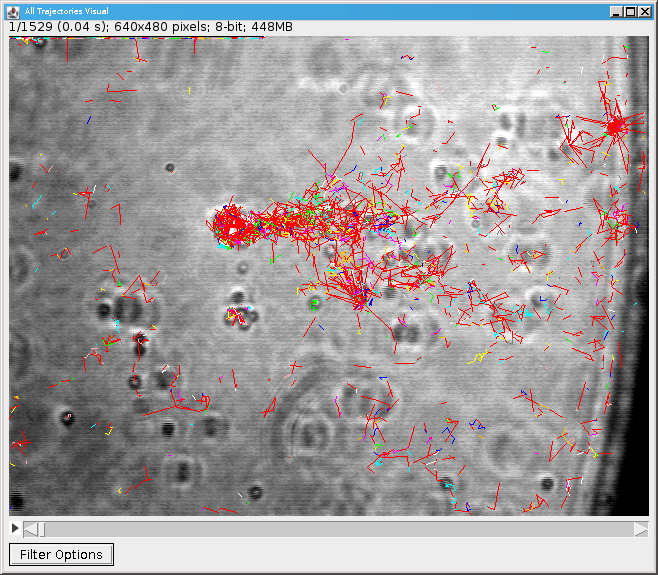
\includegraphics[width=.95\linewidth]{./figures/traj_petit_trap}
	\caption{small particles trapped}
	\label{fig:test1}
\end{minipage}%
\begin{minipage}{.5\textwidth}
	\centering
	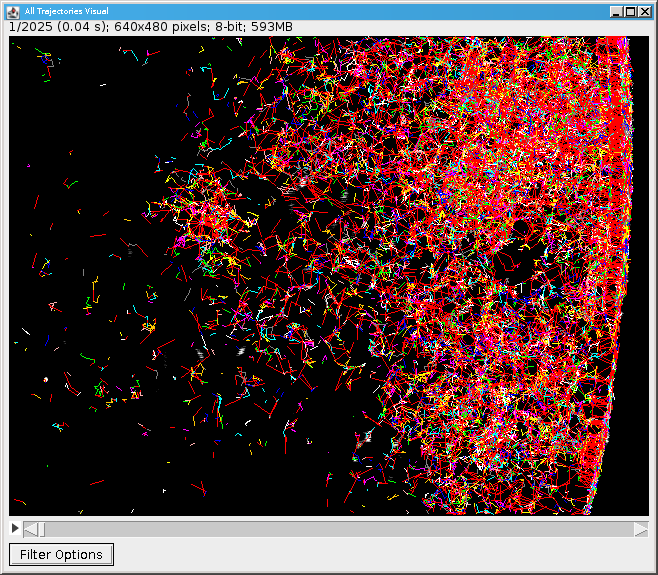
\includegraphics[width=.95\linewidth]{./figures/traj_petit_free}
	\caption{small particles free}
	\label{fig:test2}
\end{minipage}
\end{figure}


\begin{figure}
	\begin{center}
	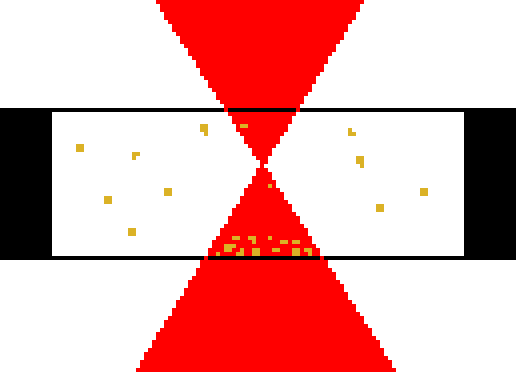
\includegraphics[width=0.7\linewidth,angle=0]{./figures/trap_illustration}
	\caption{we suspect that particles are trapped like in this illustration} \label{fig:gros_trap}
	\end{center}
\end{figure}

We wrote a program that takes the output of the MOSAIC plugin for imageJ as input, so that we can get the average diffusion coefficient and the force applied on the particle when the beam is activated.


% \clearpage

% - expliquer les calculs

% - le trap selon x y : montrer que ca marche

% - le trap selon z : expliquer

% le plus important!!!

\section{Conclusion}

Even with no quantitative evaluation of the result of the experiment, it was clear that the trapping on x and y was working greatly, it was possible with ease to move a particle, or even a group of particles anywhere on the plate with a high velocity without loosing it/them. However, there was that problem that there was no control on z, and that the lens were not the one expected that worked the best. It might be interesting to get a way to measure the z position of a particle with the knowledge of the lenses used in the system and the way the particle appear blurry, since they all looked like rings, it might not be extremely hard to track that kind of shape. This might allow some deeper analysis on the way those particle are moving.






\end{document} %%%% THE END %%%%


